\documentclass{oblivoir}
\usepackage{amsmath,amssymb,amsthm,kotex,mdframed,paralist,kswrapfig}

\newcounter{num}
\newcommand{\prob}
{\bigskip\noindent\refstepcounter{num}\textbf{문제 \arabic{num})}\par}

\newcommand{\ans}{{\raggedleft\textbf{답 : (\qquad\qquad\qquad\qquad\qquad\qquad)}
\par}\bigskip\bigskip}


\newcommand\ga{\text{(가)}}
\renewcommand\na{\text{(나)}}


%%%
\begin{document}
\Large

\title{승재 13 - 6학년 2학기 - 06}
\author{}
\date{\today}
\maketitle
%\tableofcontents

\newpage

%
\prob
다음 \(\square\)에 들어갈 알맞은 숫자를 쓰세요.

\begin{enumerate}[(1)]
\item
\(5:2=\square:\frac47\)
\item
\(4:\frac15=2:\square\)
\item
\(\frac12:\frac13=12:\square\)
\item
\(\frac29:2=4:\square\)
\item
\(1:\frac34=\frac34:\square\)
\item
\(\frac76:\frac52=\square:10\)
\item
\(\frac{40}3:\frac{75}2=\square:\frac{15}2\)
\item
\(\frac{10}7:\frac{12}5=\square:\frac{98}{15}\)
\item
\(\frac{13}2:52=\square:4\)
\item
\(\frac{36}5:7=\frac{12}7:\square\)
\item
\(4.9:2.8=14:\square\)
\item
\(1.21:1.43=\square:26\)
%\item
%\(85:80=3.4:\square\)
\item
\(3.14:12.56=5:\square\)
\item
\(7.17:3=16.73:\square\)
\item
\(200:1500=0.8:\square\)
\item
\(400:150=0.16:\square\)
\item
\(270:126=\frac94:\square\)
\item
\(5.68:14.2=\square:\frac27\)
\item
\(5.88:56=\frac{14}3:\square\)
\end{enumerate}

%
\prob

다음 \(\square\), \(\triangle\)에 들어갈 알맞은 숫자를 구하고 풀이과정을 적으세요.
\[1:2:4=\square:16:\triangle\]
\begin{mdframed}
\textbf{풀이 : }
전항과 후항으로 이루어져 있는 비례식과는 달리 세 개의 항으로 이루어진 비례식입니다.
이 때, \(1:2=\square:16\)과 \(2:4=16:\triangle\)이 성립하게 됩니다.
따라서 \(\square=8\), \(\triangle=32\)입니다.
\end{mdframed}

{\raggedleft\textbf{답 : (\quad\(\square\)=8,\quad \(\triangle\)=32\quad)}
\par}\bigskip\bigskip

%
\prob
다음 \(\square\), \(\triangle\)에 들어갈 알맞은 숫자를 구하고 풀이과정을 적으세요.
\[3:4:5=12:\square:\triangle\]
\begin{mdframed}
\textbf{풀이 : }
\vspace{0.3\textheight}
\end{mdframed}

\ans

%
\prob
다음 \(\square\), \(\triangle\)에 들어갈 알맞은 숫자를 구하세요.
\begin{enumerate}[(1)]
\item
\(2:3:5=\square:\triangle:25\)
\item
\(2:6:7=\square:\triangle:14\)
\item
\(4:2:3=\square:8:\triangle\)
\item
\(5:8:6=\square:\frac43:\triangle\)
\item
\(2:7:4=4:\square:\triangle\)
\item
\(3:1:4=6.3:\square:\triangle\)
\end{enumerate}

%
\prob
준수와 혜리와 윤주가 색연필 45자루를 2:3:4로 나누어 가지려고 합니다.
준수와 혜리와 윤주가 가지게 되는 색연필은 각각 몇 자루입니까?

{\raggedleft\textbf{
답 :
준수 (\qquad\qquad\qquad\qquad)\\
혜리 (\qquad\qquad\qquad\qquad)\\
윤주 (\qquad\qquad\qquad\qquad)\\
}
\par}\bigskip\bigskip

%
\prob
경민이가 가진 지우개, 연필, 자의 길이의 비는 3:7:8입니다.
연필의 길이가 8.4cm일 때, 지우개와 자의 길이의 합을 구하세요.

\ans

\newpage

%
\prob
가로, 세로, 높이의 비가 2:3:5인 직육면체가 있습니다.
이 직육면체의 모서리의 길이의 합이 120cm일 때, 이 직육면체의 부피를 구하세요.
\begin{figure}[h!]
\centering
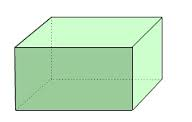
\includegraphics{parallelopipedon}
\end{figure}

\ans

%
\prob
(가)의 0.35는 (나)의 \(\displaystyle\frac27\)과 같을 때 (가) : (나)를 가장 간단한 자연수의 비로 나타내고, 그 풀이과정을 쓰세요.
\begin{figure}[h]
\centering
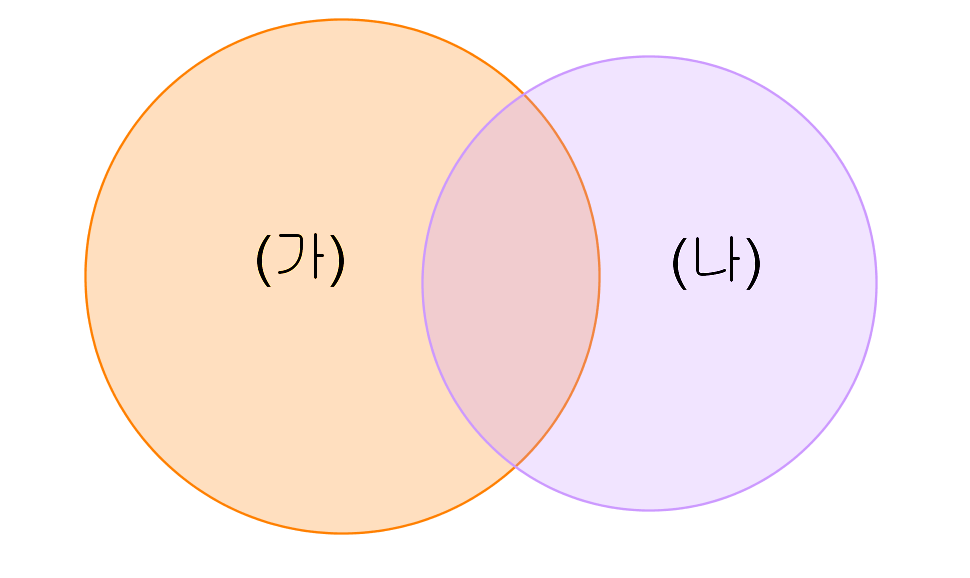
\includegraphics[width=0.5\textwidth]{09}
\end{figure}
\begin{mdframed}
\textbf{풀이 : }
\vspace{0.3\textheight}
\end{mdframed}

\ans

%
\prob
(가) : (나)를 가장 간단한 자연수의 비로 나타내고 그 풀이과정을 쓰세요.
\[
\ga\times1.8=\na\times2.2
\]
\begin{mdframed}
\textbf{풀이 : }
\vspace{0.3\textheight}
\end{mdframed}
\ans




%
\prob
민희와 효연이는 바나나를 먹었습니다.
민희는 큰 바나나 2개를 먹었고 효연이는 큰 바나나 1개, 작은 바나나 4개를 먹었습니다.
민희와 효연이가 먹은 바나나의 양을 가장 간단한 자연수의 비로 나타내세요.
(단, 큰 바나나의 크기는 작은 바나나의 크기의 세 배입니다.)

\begin{figure}[h!]
\centering
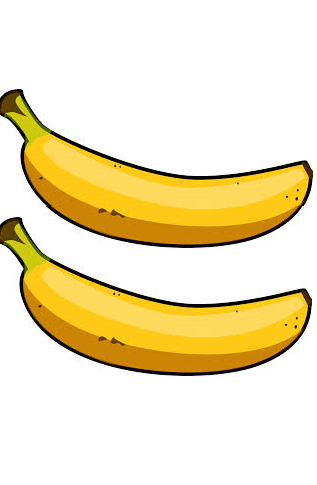
\includegraphics[width=0.4\textwidth]{01-1}
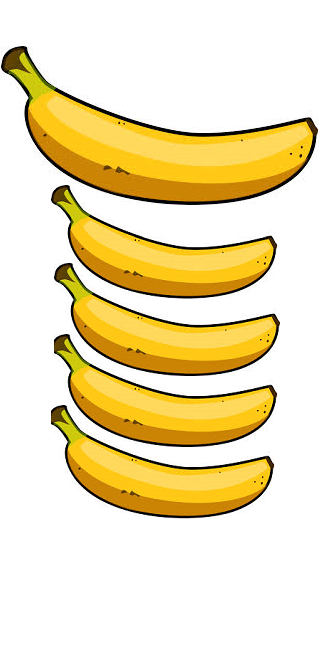
\includegraphics[width=0.4\textwidth]{01-2}

민희가 먹은 바나나 \qquad\qquad\quad 효연이가 먹은 바나나
\end{figure}

\ans

\newpage

%
\prob
지호와 영신이는 바나나를 먹었습니다.
지호는 큰 바나나 2개, 작은 바나나 3개를 먹었고
영신이는 큰 바나나 1개, 작은 바나나 4개를 먹었습니다.
지호와 영신이가 먹은 바나나의 양을 가장 간단한 자연수의 비로 나타내세요.
(단, 큰 바나나의 크기와 작은 바나나의 크기의 비는 3:2입니다.)

\begin{figure}[h!]
\centering
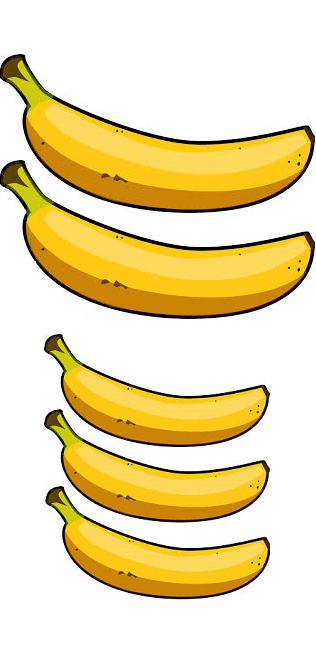
\includegraphics[width=0.4\textwidth]{02-1}
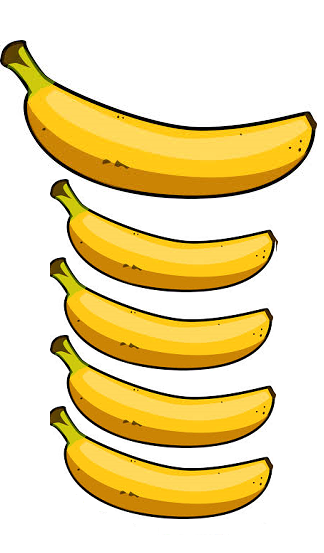
\includegraphics[width=0.4\textwidth]{02-2}

\qquad지호가 먹은 바나나\qquad\qquad\quad 영신이가 먹은 바나나
\end{figure}

\ans

\newpage

%
\prob
지수는 큰 바나나 3개를 먹었고 효정이는 작은 바나나 4개를 먹었습니다.
지수와 효정이가 먹은 바나나의 양은 서로 같을 때, 큰 바나나와 작은 바나나의 크기의 비를 가장 간단한 자연수의 비로 나타내세요.

\begin{figure}[h!]
\centering
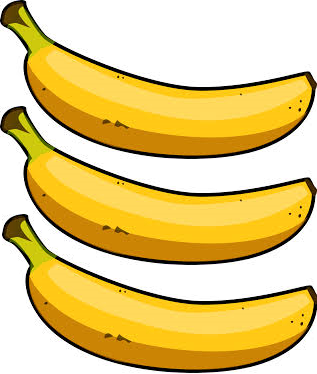
\includegraphics[width=0.4\textwidth]{03-1}
\qquad\qquad
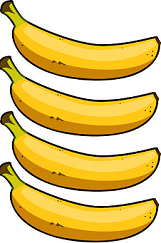
\includegraphics[width=0.3\textwidth]{03-2}

\qquad지수가 먹은 바나나\qquad\qquad\qquad\quad 효정이가 먹은 바나나
\end{figure}

\ans

\newpage

%
\prob
윤지는 큰 바나나 2개와 작은 바나나 5개를 먹었고 준호는 큰 바나나 4개와 작은 바나나 2개를 먹었습니다.
윤지와 준호가 먹은 바나나의 양은 서로 같을 때, 큰 바나나와 작은 바나나의 크기의 비를 가장 간단한 자연수의 비로 나타내세요.

\begin{figure}[h!]
\centering
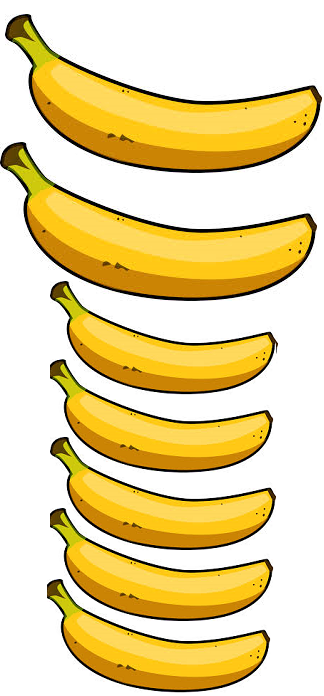
\includegraphics[width=0.4\textwidth]{04-1}
\qquad\qquad
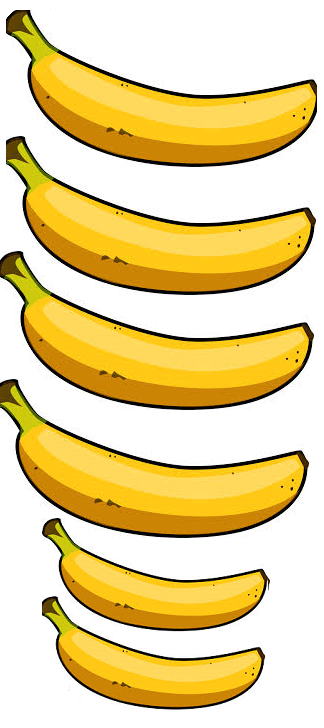
\includegraphics[width=0.4\textwidth]{04-2}

\qquad윤지가 먹은 바나나\qquad\qquad\qquad\quad 준호가 먹은 바나나
\end{figure}

\ans

\newpage

%
\prob
가로의 길이가 5cm, 세로의 길이가 3cm인 직사각형의 바깥쪽으로 반지름이 1cm인 원이 한 바퀴 굴러 제자리로 돌아올 때, 이 원이 지나간 자리를 그림으로 표시하고 그 넓이를 구하세요.

\begin{figure}[h!]
\centering
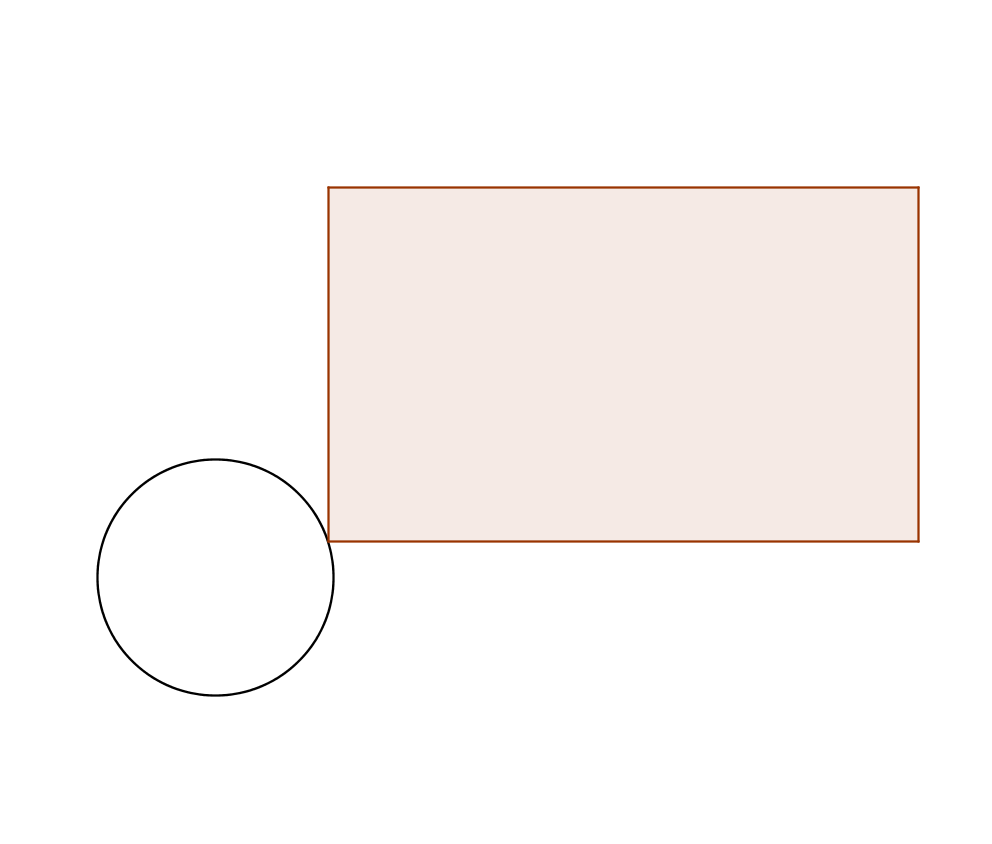
\includegraphics[width=0.45\textwidth]{rectangle-circle}
\end{figure}

\ans

%
\prob
한 변의 길이가 4cm인 정사각형의 바깥쪽으로 반지름이 1cm인 원이 한 바퀴 굴러 제자리로 돌아올 때, 이 원이 지나간 자리를 그림으로 표시하고 그 넓이를 구하세요.
\begin{figure}[h!]
\centering
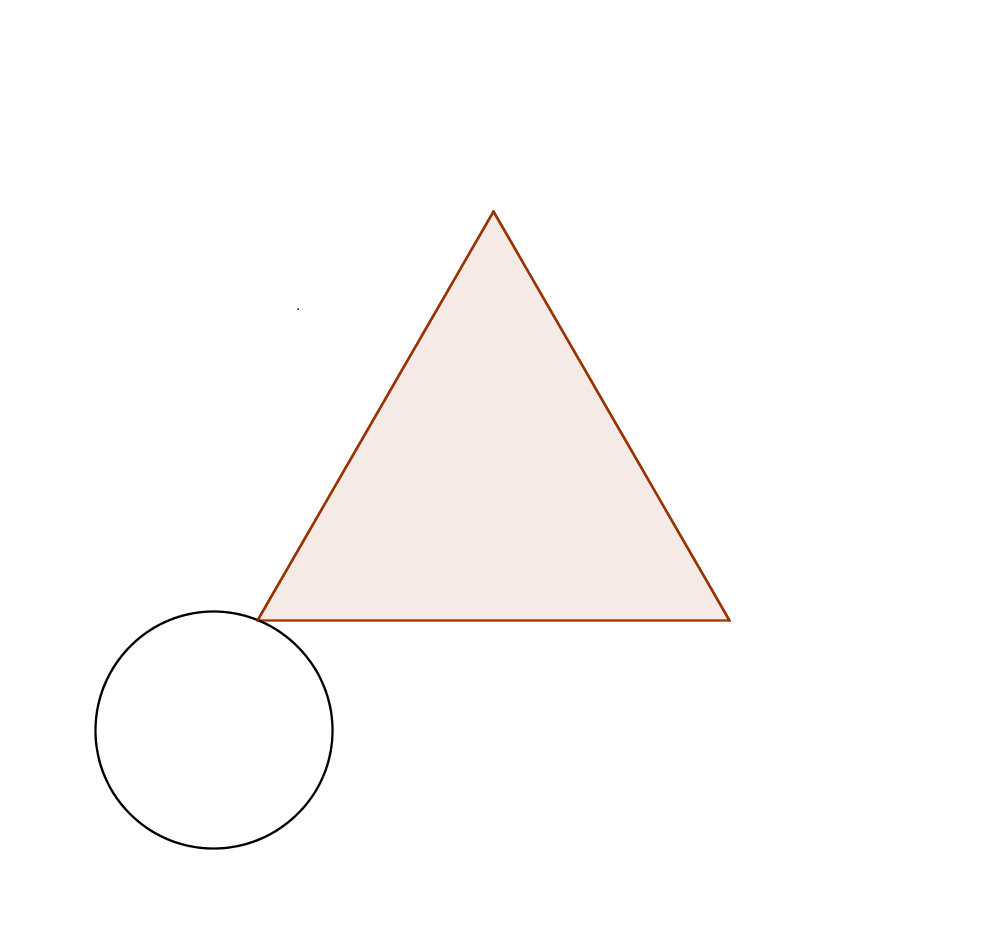
\includegraphics[width=0.45\textwidth]{triangle-circle}
\end{figure}

\ans

%
\prob
아래 그림은 한 변의 길이가 20cm인 원의 1/4 안에 들어가는 정사각형을 표현한 것입니다.
이 도형의 넓이를 구하세요.
\begin{figure}[h!]
\centering
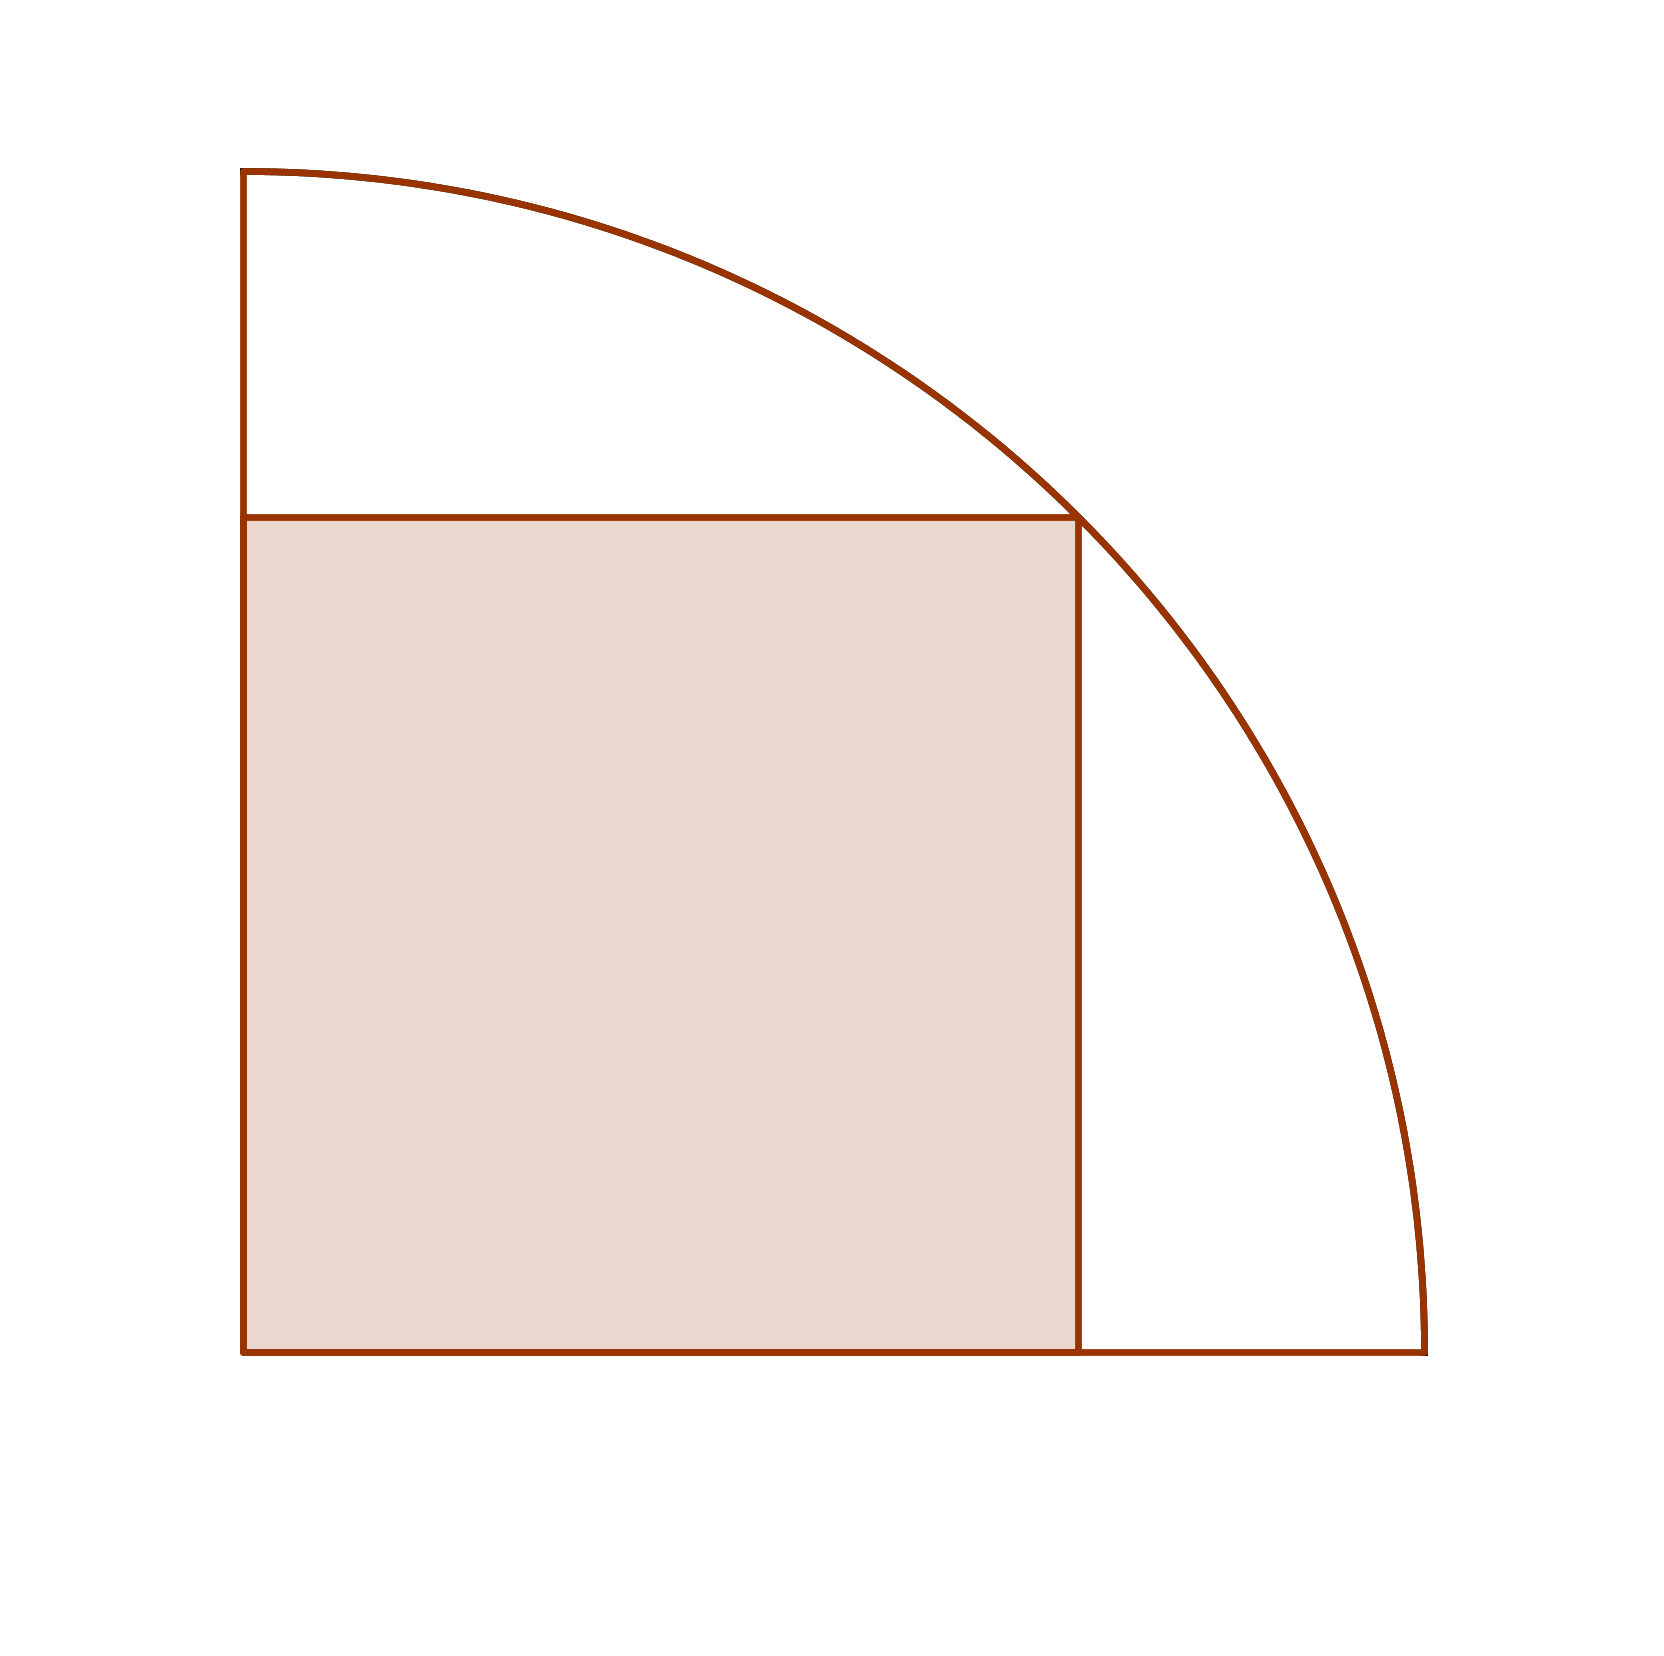
\includegraphics[width=0.5\textwidth]{quadrant}
\end{figure}

\ans

%
\prob
다음 마름모의 넓이를 구하세요.

\begin{figure}[h!]
\centering
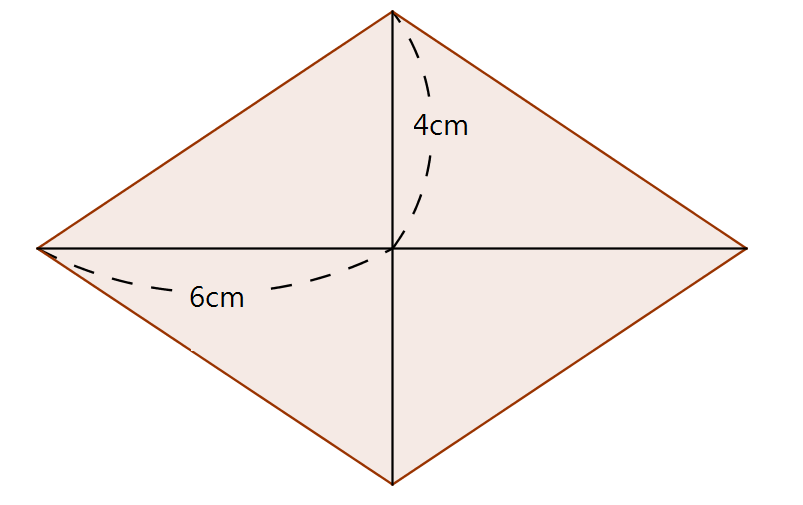
\includegraphics[width=0.5\textwidth]{rhombus}
\end{figure}
\ans
\end{document}